\documentclass[10pt,twocolumn,twoside]{IEEEtran}

\usepackage{afterpage}
\usepackage{bold-extra}
\usepackage{color}
\usepackage{float}
\usepackage{graphicx}
\usepackage{listings}
\usepackage{subfigure}

%%%%%%%%%%%%%%%
%%% Colours %%%
%%%%%%%%%%%%%%%

\definecolor{darkgreen}{rgb}{0, 0.6, 0}
\definecolor{lightgrey}{gray}{0.9}

%%%%%%%%%%%
% Figures %
%%%%%%%%%%%

% Define shorter ways to include individual images
\newcommand{\stufig}[4]						% images with default placement
{
	\begin{figure}
	\begin{center}
		\includegraphics[#1]{#2}
		\caption{#3}
		\label{#4}
	\end{center}
	\end{figure}
}

\newcommand{\stufigex}[5]					% images with specified placement
{
	\begin{figure}[#5]
	\begin{center}
		\includegraphics[#1]{#2}
		\caption{#3}
		\label{#4}
	\end{center}
	\end{figure}
}

\newcommand{\stufigexx}[5]				% full-width images with specified placement
{
	\begin{figure*}[#5]
	\begin{center}
		\includegraphics[#1]{#2}
		\caption{#3}
		\label{#4}
	\end{center}
	\end{figure*}
}

% Define the stusubfig environment
\newenvironment{stusubfig}[1]
{
	\begin{figure*}[#1]
	\begin{center}
}
{
	\end{center}
	\end{figure*}
}

%%%%%%%%%%%%%%%%%
% Code Listings %
%%%%%%%%%%%%%%%%%

% Create a new type of float (called a stulisting) for listings
\floatstyle{ruled}
\newfloat{stulisting}{thp}{lop}
\floatname{stulisting}{Listing}

% Setup before using the listings package
\renewcommand{\lstlistingname}{\textbf{Listing}}
\def\thelstlisting{\textbf{\arabic{lstlisting}}}

\lstdefinelanguage{Pseudocode}{
morekeywords={and,assert,break,case,continue,default,down,each,else,for,function,if,not,null,or,rangeswitch,ref,return,switch,then,this,throw,to,up,var,while},
sensitive=true,
morecomment=[l]{//},
morecomment=[s]{/*}{*/}
}

\lstdefinestyle{Default}{
abovecaptionskip=0.5cm,
basicstyle=\scriptsize\ttfamily,
belowcaptionskip=0.5cm,
belowskip=0.5cm,
columns=fixed,
%commentstyle=\color{darkgreen},
commentstyle=\textit, % changed from the thesis (green text looks unprofessional in a journal paper)
language=Pseudocode,
%numbers=left,
numbers=none, % changed from the thesis (line numbers are less relevant here)
numbersep=5pt,
numberstyle=\tiny,
mathescape=true,
showstringspaces=false,
stepnumber=1,
tabsize=4
}

\lstdefinestyle{Snippet}{
abovecaptionskip=0.5cm,
aboveskip=0.5cm,
basicstyle=\small\ttfamily,
belowcaptionskip=0.5cm,
belowskip=0.5cm,
columns=fixed,
commentstyle=\color{darkgreen},
frame=lines,
keywordstyle=\small\bfseries,
language=Pseudocode,
numbers=none,
mathescape=true,
showstringspaces=false,
stepnumber=1,
tabsize=4
}

% For C++ function prototypes
\lstdefinestyle{Prototype}{
abovecaptionskip=0.5cm,
basicstyle=\small\ttfamily,
belowcaptionskip=0.5cm,
belowskip=0.5cm,
columns=fixed,
commentstyle=\color{darkgreen},
language=C++,
numbers=none,
mathescape=true,
showstringspaces=false,
stepnumber=1,
tabsize=4
}

%%%%%%%%%%%%%%%%%
% Main Document %
%%%%%%%%%%%%%%%%%

\begin{document}

\title{Two Tree-Based Algorithms for the Waterfall}
\author{Stuart Golodetz, Chris Nicholls, Irina Voiculescu and Stephen Cameron}
\date{\today}
\maketitle

\begin{abstract}
\noindent TODO
\end{abstract}

%#####################
\section{Introduction}
%#####################

TODO: \cite{golodetz11}

\bibliographystyle{alpha}
\bibliography{existingwork,mypapers}

\vspace{3cm}

\begin{IEEEbiography}[{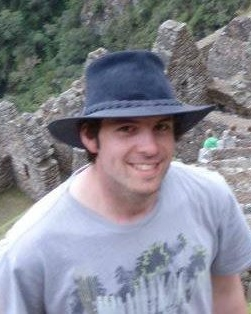
\includegraphics[width=1in,height=1.25in,clip,keepaspectratio]{pic_stuart.jpg}}]{Stuart Golodetz}
Stuart Golodetz obtained his DPhil in Computer Science at Oxford University, working on 3D image segmentation and feature identification. He then spent two interesting years in industry, working in the areas of credit risk management, logic programming and software analytics. His areas of interest include medical image analysis, computer games development and the intricacies of different programming languages, especially C++. He was a session chair for the 6th International Symposium on Image and Signal Processing and Analysis, ISPA 2009. He is a member of the Association of C and C++ Users (ACCU) and has written a number of articles for their magazines.
\end{IEEEbiography}

\begin{IEEEbiography}[{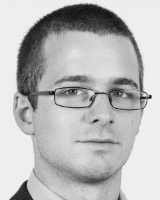
\includegraphics[width=1in,height=1.25in,clip,keepaspectratio]{pic_chris.jpg}}]{Chris Nicholls}
TODO
\end{IEEEbiography}

\begin{IEEEbiography}[{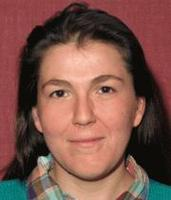
\includegraphics[width=1in,height=1.25in,clip,keepaspectratio]{pic_irina.jpg}}]{Irina Voiculescu}
TODO
\end{IEEEbiography}

\begin{IEEEbiography}[{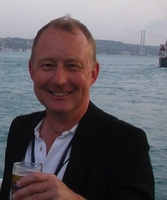
\includegraphics[width=1in,height=1.25in,clip,keepaspectratio]{pic_stephen.jpg}}]{Stephen Cameron}
Stephen Cameron obtained his PhD in Artificial Intelligence at Edinburgh University, working on the geometric modelling of robots and on collision detection. His general area of interest is in spatial reasoning, although this covers a wide range which includes the planning of tasks and motions for robot vehicles and manipulators, the use of geometric models, and the scheduling of fleets of robots. Some of his work is in collaboration with members of the Oxford University Robotics Research Group in the Department of Engineering Science. He is a member of the AISB, the IEEE Robotics and Automation Society, the Geometric Modelling Society, the IAM and CAMRA.
\end{IEEEbiography}

\end{document}
